\documentclass[FM,Proj]{tulthesis}

% 1) odhad stavů 2) odhad náročnosti 3) rešerše stávajících systémů -> klíčové fce


% tento dokument používá balíky specifické pro XeLaTeX a lze jej přeložit
% jen XeLaTeXem, nemáte-li instalována použitá (komerční) písma, změňte
% nebo vymažte příkazy \set...font na následujících řádcích

% Autor šablony: Pavel Satrapa: http://www.nti.tul.cz/~satrapa/vyuka/latex-tul/

% Autor komentářů, jejich překladů do EN, nastavení BibLaTeXu a aplikace ČSN ISO 690: Jan Koprnický
% http://www.fm.tul.cz/personal/jan.koprnicky

% ENGLISH EXPLANATION
% \documentclass[FM,Dis,EN,fonts,bw]{tulthesis} % black and white typing, dissertation thesis at FM, written in English with using of TUL Mono font
% this document uses packages specific for XeLaTeX and it is possible to 
% compile it by XeLaTeX only, if you haven't installed used (commercial) fonts
% change them or erase commands \set...font in following rows
% settings: FM (faculty: FS, FT, FP, EF, FA, FM, FZS a CXI), Dis (type of thesis: BP, DP, Teze, Autoref, Hab, SP, Proj), EN (written in English language), fonts (activation of TUL fonts), bw (black and white)

% Autor of the template tulthesis: Pavel Satrapa: http://www.nti.tul.cz/~satrapa/vyuka/latex-tul/

% Autor of several comments and their translation into English, BibLaTeX settings and CSN ISO 960 citation standard setting: Jan Koprnický
% http://www.fm.tul.cz/personal/jan.koprnicky

% poslední změna / last modification 12. 5. 2023

\newcommand{\verze}{2.0}

\usepackage{polyglossia}
\setdefaultlanguage{czech} % comment when English is preferred
%\setdefaultlanguage{english} % comment when Czech is preferred


\usepackage{makeidx}
\makeindex

\usepackage{plantuml}
\usepackage{xunicode}
\usepackage{xltxtra}
\usepackage{tikz}
\usepackage{bbding}
\usepackage{graphicx}
\usepackage{float}
\graphicspath{ {./img}{./tultex} }

% příkazy specifické pro tento dokument / specific commands for this document
\newcommand{\argument}[1]{{\ttfamily\color{\tulcolor}#1}}
\newcommand{\argumentindex}[1]{\argument{#1}\index{#1}}
\newcommand{\prostredi}[1]{\argumentindex{#1}}
\newcommand{\prikazneindex}[1]{\argument{\textbackslash #1}}
\newcommand{\prikaz}[1]{\prikazneindex{#1}\index{#1@\textbackslash #1}}
\newenvironment{myquote}{\begin{list}{}{\setlength\leftmargin\parindent}\item[]}{\end{list}}
\newenvironment{listing}{\begin{myquote}\color{\tulcolor}}{\end{myquote}}
\sloppy

% deklarace pro titulní stránku / title page declaration
\TULtitle{Návrh a analýza procesu modernizace školního informačního systému pro střední školu}{}
\TULauthor{Daniel Adámek}

% pro bakalářské, diplomové a disertační práce / for bachelor, master theses and dissertation
\TULprogramme{B0613A140005}{Informační technologie}{Information technology}
\TULbranch{}{Aplikovaná informatika}{Applied Informatics}
%\TULbranch{1802T008}{Nějaký jiný obor}{Some other branch}
\TULsupervisor{Ing. Lenka Kostková-Třísková Ph.D.}
\TULyear{2024}

% pro habilitační práce / habilitation thesis
%\TULbranch{}{Technická kybernetika}{Technical cybernetics}
%\TULyear{2022}

% Použití bibLateXu, pracuje s ISO stylem
% BibLaTeX settings, works with ISO style
\usepackage[ 
    backend=biber
    % ,style=iso-authoryear % styl vyžaduje FZS TUL , místo příkazu \cite{} je potřeba využít \parencite{} (sazba kulatých závorek) / style required by FZS TUL use \parencite{} instead of \cite{}
    ,style=iso-numeric
    %,style=numeric
    %,sortlocale=cs_CZ
    ,autolang=other
    ,bibencoding=UTF8
    %,urldate=edtf
    ,maxcitenames=2 %maximum v textu citovaných jmen
    ,maxbibnames=3 %maximum v seznamu vyjmenovaných autorů
    ]{biblatex}

\addbibresource{refs.bib}% vložení seznamu literárních zdrojů v bib formátu / input of references in bib format

% Úprava iso-numeric.bbx v souladu s požadavky TUL hranaté závorky v číslovaném seznamu / Modification of iso-numeric.bbx in accordance with TUL requirements of square brackets in a numbered list
\DeclareFieldFormat{labelnumberwidth}{\mkbibbrackets{#1}}

% Formátování podle pokynů FZS, při využití stylu iso-authoryear, čárka mezi jmény a poslední jméno se spojkou a / special requirements of FZS TUL 
\DeclareDelimFormat{multinamedelim}{\addcomma\space}

\DeclareDelimFormat{finalnamedelim}{%
  \ifnumgreater{\value{liststop}}{2}{\finalandcomma}{}%
  \addspace\bibstring{and}\space}

\DeclareNameAlias{author}{family-given/given-family} 
%%%%%%%%%%%%%%%%%%%%%%%%%%

\usepackage{csquotes} %užití biblatexu hlasí warnings, důvodem může být použití českých uvozovek v citacích! / solving of problems with Czech quotations
\urlstyle{same} %sazba url odkazů stejným fontem jako ostatní text, řešení problémů v zalamování hypertextových odkazů v citacích / url in references setting into the same form as text 


\begin{document}

\ThesisStart{female}
%\ThesisStart{zadani-a-prohlaseni.pdf}

\begin{abstractCZ}
Cílem této práce analýza současného informačního systému střední průmyslové školy, včetně popisu jeho provozu, databázového modelu, client-side scripting, server-side scripting, funkcí API a uživatelského rozhraní. Následuje analýza a porovnání komerčních a open source řešení dostupných na trhu, včetně zhodnocení výhod a nevýhod in-house vývoje informačního systému. Práce dále zahrnuje identifikaci a analýzu potřeb koncových uživatelů - zaměstnanců školy i žáků, kteří budou systém používat pro zápis známek a další agendu.

Na základě získaných informací a provedených analýz bude formulován návrh informačního systému, včetně procesu modernizace, který bude reflektovat identifikované potřeby uživatelů a moderní trendy v IT. Práce tak přispěje k lepšímu pochopení a řešení problémů současného informačního systému ve školství a poskytne návrhy na jeho zlepšení a modernizaci.
\end{abstractCZ}

\begin{keywordsCZ}
informační systém, analýza, in-house vývoj, školství
\end{keywordsCZ}

\vspace{2cm}

\begin{abstractEN}
The aim of this thesis is to analyze the current information system of a secondary industrial school, including a description of its operation, database model, client-side scripting, server-side scripting, API functions and user interface. This is followed by an analysis and comparison of commercial and open source solutions available on the market, including an evaluation of the advantages and disadvantages of in-house information system development. The work also includes the identification and analysis of the needs of the end users - school staff and students who will use the system to record grades and other agendas.

On the basis of the information obtained and the analyses carried out, a proposal for the information system will be formulated, including the modernisation process, which will reflect the identified needs of the users and modern trends in IT. The work will thus contribute to a better understanding and solution of the problems of the current information system in education and provide suggestions for its improvement and modernization.
\end{abstractEN}

\begin{keywordsEN}
information system, analysis, in-house development, education
\end{keywordsEN}

\clearpage

\begin{acknowledgement}
Prvně bych rád vyjádřil svou nejhlubší vděčnost Střední průmyslové
škole elektrotechnické, Praha 2, Ječná 30, kterou zastupuje 
ředitel Ing. Bc. et Bc. Ondřej Mandík ING-PAED IGIP. Bez 
jeho laskavosti a podpory by toto dílo nebylo možné realizovat. 
Škola mi poskytla nezbytné informace, umožnila mi analyzovat svůj 
informační systém a vytvořit nový návrh. Tato zkušenost byla pro mě 
nesmírně cenná a pomohla mi v mnoha studijních i pedagogických aspektech.

Zvláštní poděkování patří všem zaměstnancům školy a mým kolegům 
pedagogům, kteří mi pomohli kritickým pohledem na stávající 
systém a při hledání nových, lepších řešení. Jejich nápady a 
zpětná vazba byly jedním z klíčových aspektů pro vytvoření nového 
informačního systému, který je nejen efektivní, ale také nabízí 
vynikající uživatelský zážitek. Děkuji za vaši tvořivost, 
trpělivost a neocenitelnou spolupráci.

Dále bych chtěl poděkovat všem členům mého vedení, rodině a 
přátelům, kteří mi poskytli cennou pomoc a podporu během procesu 
vytváření tohoto bakalářského projektu. Jejich trpělivost, 
porozumění a povzbuzování bylo pro mě během celého procesu klíčové.

Nakonec bych chtěl vyjádřit svou vděčnost všem, kteří se na tomto 
díle podíleli, ať už přímo nebo nepřímo. Bez jejich kolektivního 
úsilí a podpory by tento projekt nebyl možný. Vaše práce a podpora
byla nesmírně cenná a jsem vám za to hluboce vděčný.

Děkuji všem.
\end{acknowledgement}

\tableofcontents

\clearpage

\begin{abbrList}
\textbf{FM TUL} & Fakulta mechatroniky, informatiky a mezioborových studií
Technické univerzity v~Liberci \\
\textbf{SPŠE Ječná} & Střední průmyslová škola elektrotechnická, Praha 2, Ječná 30 \\
\textbf{IS} & Informační systém \\
\textbf{ŠIS} & Školní informační systém \\
\textbf{SŘBD} & Systém řízení báze dat \\
\textbf{SSR} & Server side rendering \\
\textbf{CSR} & Client side rendering \\
\textbf{LDAP} & Lightweight Directory Access Protocol \\
\textbf{VPS} & Virtual Private Server \\
\textbf{DDoS} & Distributed Denial of Service \\
\textbf{SPU} & Specifické poruchy učení \\
\textbf{MŠMT} & Ministerstvo školství, mládeže a tělovýchovy
\end{abbrList}

\chapter{Uvedení do problematiky a stanovení cílů práce}
\section{Představení tématu}

Informační systémy (IS) hrají zásadní roli ve všech oblastech moderního
života a jejich význam se neustále zvyšuje. Školství, jakožto oblast 
s velkým množstvím různých typů informací potřebných ke správnému 
fungování, je obzvláště závislé na efektivních řešení. Přestože školské 
IS již mají dlouhou historii, jejich vývoj pokračuje a je ovlivněn nejen 
novými technologiemi, ale také změnami v požadavcích uživatelů a zákonodárství.

Tento bakalářský projekt se zaměřuje na problematiku modernizace současného 
školního IS, který slouží ke správě široké školy aspektů vzdělávacího procesu. 
Současný systém pokrývá různé oblasti, včetně: správy žáků, tříd, zaměstnanců, 
známek, certifikací k maturitní zkoušce, tématických plánů a dalších klíčových 
prvků školní administrativy. Přestože tento systém funguje a plní svou úlohu, 
existuje potřeba jeho modernizace a zlepšení, aby odpovídal současným trendům 
a potřebám, které se každoročně mění.

Následující práce se bude zabývat podrobnou analýzou tohoto systému, 
identifikací jeho slabých míst a možností zlepšení. Na základě této analýzy 
bude formulován návrh modernizace systému, který zohlední jak technologické 
možnosti, tak potřeby a preference uživatelů. Cílem práce je nejen teoretický 
přínos v podobě podrobného zkoumání jednoho konkrétního systému, ale také 
praktický přínos v podobě návrhu konkrétních krokl pro zlepšení systému a 
tím kvality služeb poskytovaných školou.

\section{Stanovení cílů a otázek práce}
Cíle tohoto bakalářského projektu jsou pečlivě vybrány tak, aby co 
nejkomplexněji pokrývaly klíčové aspekty analýzy, návrhu a modernizace školního 
IS. Hlavním cílem je provést důkladnou analýzu stávajícího systému, včetně 
jeho provozu, databázového modelu, klientové a serverové skriptování, funkcí 
API a uživatelského rozhraní. Tato analýza poskytne hluboké porozumění současnému
stavu a odhalí možné nedostatky a oblasti pro zlepšení.

Dalším cílem je provést podrobný přezkum a srovnání komerčních a open source řešení
dostupných na trhu, a posoudit výhody a nevýhody interního vývoje IS. Tato část 
práce poskytne cenný vhled do dostupných možností a pomůže při formulaci 
návrhu nového systému.

Na základě stanovených cílů jsem vytyčil několik klíčových otázek, které 
jsou základním kamenem pro pochopení tématu a slouží jako orientační body pro tento 
projekt. Každá otázka je zaměřena na specifický aspekt problematiky a její 
zodpovězení nám umožní dospět k uceleným závěrům a vyvodit praktické doporučení. 
Detailní rozbor těchto otázek je následující:

\begin{enumerate}
\item \textit{Jak je strukturován a jak funguje současný ŠIS?} 
Cílem této otázky je získat komplexní porozumění fungování stávajícího systému, 
jeho architektury, funkcí a procesů, které podporuje. To zahrnuje analýzu 
databázového modelu, klientové a serverové skriptování, funkcí API a uživatelského rozhraní.

\item \textit{Jaké jsou hlavní nedostatky současného systému z pohledu koncových uživatelů?}
 Odpověď na tuto otázku nám umožní identifikovat slabé stránky současného systému a 
 určit klíčové oblasti pro zlepšení. Zohlednění pohledu koncových uživatelů je 
 klíčové pro návrh efektivního a uživatelsky přívětivého systému.

\item \textit{Jaká komerční a open source řešení jsou dostupná a jak se porovnávají s 
interním vývojem?} Tato otázka je zaměřena na průzkum trhu a srovnání různých dostupných 
řešení. To nám poskytne přehled o tom, jaké možnosti máme k dispozici a umožní nám vybrat 
nejvhodnější řešení pro naše potřeby.
\end{enumerate}

Tyto otázky jsou pevně zakotveny v mém výzkumném záměru a budou sloužit jako kompas 
při průzkumu složitého terénu modernizace informačních systémů ve školství.
Stanovením těchto cílů a otázek práce je položen pevný základ pro komplexní a 
systematické zkoumání tématu, což vede k hodnotným závěrům a praktickým 
doporučením pro budoucí vývoj a implementaci informačního systému.

\section{Důvod a motivace k práci}
Motivací k práci je naléhavá potřeba detailní analýzy současného informačního 
systému (IS) a vytvoření návrhu nového, aby byla zajištěna co nejúspěšnější 
modernizace školního IS. Současný systém, ačkoliv byl ve své době velmi pokrokový 
a inovativní, je nyní téměř deset let starý a začíná prokazovat známky zastarávání.

\subsection*{Stav současného systému}
Když byl systém nasazen, představoval špičkové řešení, které zpřístupnilo řadu 
moderních funkcí a nástrojů jak pro učitele, tak pro žáky. Bohužel, 
technologický vývoj neustále pokračuje, a systém, který kdysi představoval 
přední linii, nyní ztrácí krok s novými trendem v IT.

\subsection*{Hodnocení nákladů}
Nynější ředitel školy, který je původním architektem a vývojářem IS školy, avšak nově
se do vývoje přidávám já, v pozici metodika ICT. Provedli jsme analýzu stávajícího systému
a dospěli k závěru, že náklady na jeho další vývoj a údržbu by převyšovaly náklady na 
návrh a realizaci zcela nového systému. Toto hodnocení nezahrnuje pouze finanční aspekt,
ale také čas a lidské zdroje, které by byly potřebné pro přizpůsobení stávajícího systému
 novým potřebám a standardům.

\subsection*{Nové technologie a uživatelský zážitek}
Moderní technologie přinášejí nejen efektivitu, ale také vylepšují celkový uživatelský zážitek.
Nový systém by byl navržen tak, aby byla výpočetní náročnost minimalizována, což by značně 
snížilo dobu odezvy serveru. To by mělo přímý dopad na uživatelský zážitek, protože 
rychlejší odezvy znamenají plynulejší interakce a vyšší spokojenost uživatelů.

\subsection*{Ekonomická efektivita}
Snížení výpočetní náročnosti nejen zvyšuje efektivitu a uživatelskou spokojenost, ale 
také vede k snížení nákladů na provoz serveru. Nový systém by byl optimalizován tak, 
aby co nejvíce šetřil zdroje, čímž by se dosáhlo úspor nejen v oblasti hardwarových nákladů,
ale také v energetické spotřebě.

\subsection*{Závěr}
Modernizace stávajícího IS na střední škole není jen otázkou technologického pokroku.
Je to komplexní úkol, který vyžaduje pečlivé zvážení řady faktorů, včetně finančních, 
technologických, uživatelských potřeb a dlouhodobé udržitelnosti. Tato práce se pokusí 
poskytnout komplexní pohled na tyto aspekty a představit cestu, jak dosáhnout nejen 
technologické excelence, ale také ekonomické efektivnosti a udržitelnosti v moderním 
vzdělávacím prostředí.

\chapter{Teoretický rámec}
V této kapitole je kladen důraz na teoretické aspekty, které formulují základ práce 
modernizace. Teoretický rámec pomáhá vytyčit parametry a omezení, ve kterých bude 
práce působit, a také poskytuje základ pro analýzu a interpretaci shromážděných dat. 

Nejdříve avšak je třeba se věnovat, pokud chceme podrobněji analyzovat IS ve vzdělávání 
a jejich návrh, definici základních problémů samotné problematiky. Definicí 
informačního systému je obecně:
\\\\
\textit{,,Informačním systémem obecně nazýváme organizaci údajů vhodnou pro systémové 
zpracování dat: pro jejich sběr, uložení a uchování, zpracování, vyhledávání a vydávání 
informací o nich, to vše pro rozhodování v běžné praxi."}\cite{Sarmanova2008ISaDS}
\\\\
Pro automatizované informační systémy:
\\\\
\textit{,,Informačním systémem automatizovaným (realizovaném na počítači) rozumíme programový 
celek, řešící rozsáhlejší oblast aplikační, naprogramovaný obvykle v jednom SŘBD s 
vhodně navrženými datovými strukturami tak, aby všechny aplikační úlohy k nim měly optimální 
přístup. Řeší uložení, uchování, zpracování a vyhledávání informací a umožňuje jejich 
formátování do uživatelsky přívětivého tvaru."}\cite{Sarmanova2008ISaDS}

\section{Obecný přehled o informačních systémech v oblasti školství}
V oblasti školství v České republice je v současné době v provozu několik školních 
IS, které slouží k efektivnímu řízení a správě školních institucí. 
Mezi nejrozšířenější IS pro základní a střední školy patří:

\begin{samepage}
    \begin{itemize}
        \item \textbf{Bakaláři:} Bakaláři je jeden z nejrozšířenějších školních informačních 
        systémů v České republice. Tento systém je výsledkem dlouholetého vývoje a je určen pro 
        základní a střední. Umožňuje komplexní správu školní agendy, od hodnocení žáků až po 
        komunikaci s rodiči. Bakaláři také nabízí mobilní aplikaci pro snadnější přístup 
        k informacím o výuce a hodnocení.

        \item \textbf{Škola OnLine:} Škola OnLine je moderní ŠIS, 
        který umožňuje zpracovávat veškerou školní agendu při zachování vysokého uživatelského 
        komfortu. Jedná se o webovou aplikaci, což znamená, že je dostupná 24 hodin denně 
        prostřednictvím Internetu, a to při využití pouze běžného webového prohlížeče 
        bez nutnosti jakékoliv další instalace.

        \item \textbf{EduPage:} Další systém, který se proslavil s době postižené onemocněním 
        COVID-19, kvůli kterému byla veškerá výuka převedena do offline formy. Tento software
        všechny potřebné služby pro výuku zahrnul na jedno místo a nebylo třeba v komunikaci 
        mezi žákem a školou potřeba využívat více služeb naráz.

    \end{itemize}
\end{samepage}

\section{Potřeby informačního systému}
Jako první je klíčové specifikovat, proč je IS 
v organizaci potřebný. V kontextu školního prostředí by měl systém 
primárně poskytovat komplexní řešení pro správu školy. Toto zahrnuje, 
ale není omezeno na, administrativní funkce, plánování rozvrhů, 
finanční správu, a další logistické aspekty.

Kromě administrativního řízení by měl IS nabízet 
pokročilé funkce pro evidence vzdělávání a vzdělávací procesy. 
Toto zahrnuje sledování žákovských výsledků, docházky, a dalších 
relevantních metrik. Efektivní analýza těchto dat může pomoci školám 
v přijímání informovaných rozhodnutí, která přispějí k celkovému 
zlepšení kvality vzdělávání.

Je rovněž důležité posoudit, co by se stalo v případě, že by nebyl 
implementován kvalitní IS. V takovém scénáři by se 
škola pravděpodobně potýkala s výzvami spojenými s neefektivní 
komunikací, zdlouhavými administrativními procesy. Absence kvalitního 
systému by mohla vést k zhoršenému rozhodování, nedostatečné 
koordinaci mezi odděleními a potenciálně i k negativním dopadům 
na vzdělávací výsledky či výchovné aspekty žáků.

\section{Teorie a koncepty spojené s informačními systémy}
Informační systémy jsou soubory lidí, procesů a technologií, které slouží k
organizování, ukládání a analýze informací. V kontextu školství jsou
IS klíčové pro efektivní správu školní agendy, od záznamů o žácích, 
známkách, absence a certifikace.

Z teoretického hlediska je vývoj IS ovlivněn několika klíčovými
koncepty, jako jsou databázové modelování, client-server architektura, a návrh speciálního
uživatelského rozhraní. Tyto koncepty se mohou promítat do různých funkcionalit, 
které by moderní školní IS měl mít. K těmto funkcionalitám patří:

\begin{itemize}
    \item \textbf{Správa žákovské agendy:} Systém by měl umožňovat snadné přidávání, úpravu a vyhledávání záznamů o žácích.
    
    \item \textbf{Organizace přijímacího řízení:} Systém by měl umožňovat organizaci přijímacího řízení vše od 
    žádosti o studium, přes přijímací zkoušky organizované společností \textbf{CERMAT - Centrum pro zjišťování 
    výsledků vzdělávání}, po konečné zavedení žáka do systému.
    
    \item \textbf{Správa dokumentů vydávaných školou:} Každý dokument vydaný školou musí mít své tzv. Jednací číslo.
    Ty generuje spisová služba dle 499/2004 Sb. Zákona o archivnictví a spisové službě. Do dokumentů, které musí mít
    své jednací číslo spadá například vysvědčení, pochvala třídního učitele či ředitele školy.

    \item \textbf{Správa známek a hodnocení:} Učitelé musí mít možnost snadno zadávat a upravovat známky, 
    a žáci by je měli snadno nalézt.

    \item \textbf{Správa SPU žáků:} Škola musí přizpůsobovat podmínky výuky všem žákům se specifickými poruchami učení
    nebo chování (SPU). Tyto posudky a celou agendu žáků s SPU spravuje školní výchovný poradce či školní psycholog.
    Informační systém by měl obsahovat posudky žáků z pedagogicko-psychologických poraden k nahlédnutí všem pedagogům, 
    kteří žáka vyučují, pro správné přizpůsobení podmínek.

    \item \textbf{Suplování:} Systém pro správu mimořádných akcí, které nejsou v řádném rozvhu třídy/skupiny/učitele.
    
    \item \textbf{Zamlouvání učeben:} Systém pro správu volných učeben pro mimoškolní akce, jako jsou kroužky, komerční
    akce, či doučování.
    
    \item \textbf{Správa žákovských skupin:} Některé předměty, jako jsou ty jazykové nebo třeba odborné, se dělí na skupiny pro 
    kontaktnější a názornější výuku.
    
    \item \textbf{Centrální evidence závad:} Systém pro snadnou evidenci závad k vyřešení.

    \item \textbf{Správa absencí:} Automatizovaný systém pro zaznamenávání absence žáků, s možností notifikace rodičů.
    
    \item \textbf{Dokumentový management:} Úložiště pro školní dokumenty, jako jsou rozvrhy, plány a interní materiály.
    
    \item \textbf{Certifikace a kvalifikace:} Sekce, kde lze evidovat různé certifikáty a kvalifikace, které žák získal.

    \item \textbf{Elektronická třídní kniha:} Systém pro správu elektronické třídnice, kde se uchovávají například data 
    o absenci žáků a probírané látce.

    \item \textbf{Správa tématických plánů:} Škola může disponovat konkrétní konkretizaci ŠVP, tedy tématických plánů,
    které plánují jednotlivé hodiny.
    
    \item \textbf{Offline režim:} Možnost pokračovat v práci i v případě, když je internetové připojení nedostupné.

    \item \textbf{Matriční záznamy:} Systém pro správu a aktualizaci dat o studujících žácích s matričním úřadem.

    \item \textbf{Responzivní design:} Vzhled webové aplikace přizpůsobený více druhům zařízení jako jsou laptopy,
    tak i pro tablety, chytré telefony i televize, či hodinky.

    \item \textbf{Mobilní aplikace:} Aplikace, která zobrazuje data z webové stránky přímo v telefonu. Často
    disponuje funkcionalitami, které na webu nejsou možné, či velmi obtížně. Příkladem mohou být notifikace.

\end{itemize}

Výběr těchto funkcionalit je založen na aktuálních potřebách školního prostředí a očekáváních koncových uživatelů,
a je navržen tak, aby splňoval moderní standardy a technologické možnosti.

\section{Přezkum a srovnání funkcionalit}

Pro efektivní srovnání funkcionalit různých ŠIS využiji tabulkovou formu. Tímto způsobem je možné jednoduše zjistit,
které z dostupných systémů nabízí funkce, jež jsou pro danou školní instituci klíčové.

\renewcommand{\arraystretch}{1.5}
\begin{table}[h]
    \begin{tabular}{lcccc}
    \hline
    \multicolumn{1}{|l|}{\textbf{FUNKCIONALITA/IS}}     & \multicolumn{1}{c|}{\textbf{Ječná IS}}                 & \multicolumn{1}{l|}{\textbf{Bakaláři}}        & \multicolumn{1}{c|}{\textbf{\begin{tabular}[c]{@{}c@{}}Škola\\ OnLine\end{tabular}}} & \multicolumn{1}{l|}{\textbf{EduPage}}                  \\ \hline
    \multicolumn{1}{|l|}{Správa žákovské agendy}        & \multicolumn{1}{c|}{{\color[HTML]{009901} \CheckmarkBold}}          & \multicolumn{1}{c|}{{\color[HTML]{009901} \CheckmarkBold}} & \multicolumn{1}{c|}{{\color[HTML]{009901} \CheckmarkBold}}                                        & \multicolumn{1}{c|}{{\color[HTML]{009901} \CheckmarkBold}}          \\ \hline
    \multicolumn{1}{|l|}{Organizace přijímacího řízení} & \multicolumn{1}{c|}{{\color[HTML]{009901} \CheckmarkBold}}          & \multicolumn{1}{c|}{{\color[HTML]{009901} \CheckmarkBold}} & \multicolumn{1}{c|}{{\color[HTML]{CB0000} \XSolid}}                               & \multicolumn{1}{c|}{{\color[HTML]{CB0000} \XSolid}} \\ \hline
    \multicolumn{1}{|l|}{Správa spisových dokumentů}    & \multicolumn{1}{c|}{{\color[HTML]{CB0000} \XSolid}}          & \multicolumn{1}{c|}{{\color[HTML]{009901} \CheckmarkBold}} & \multicolumn{1}{c|}{{\color[HTML]{CB0000} \XSolid}}                               & \multicolumn{1}{c|}{{\color[HTML]{CB0000} \XSolid}} \\ \hline
    \multicolumn{1}{|l|}{Správa známek a hodnocení}     & \multicolumn{1}{c|}{{\color[HTML]{009901} \CheckmarkBold}}          & \multicolumn{1}{c|}{{\color[HTML]{009901} \CheckmarkBold}} & \multicolumn{1}{c|}{{\color[HTML]{009901} \CheckmarkBold}}                                        & \multicolumn{1}{c|}{{\color[HTML]{009901} \CheckmarkBold}}          \\ \hline
    \multicolumn{1}{|l|}{Správa SPU žáků}               & \multicolumn{1}{c|}{{\color[HTML]{009901} \CheckmarkBold}}          & \multicolumn{1}{c|}{{\color[HTML]{CB0000} \XSolid}} & \multicolumn{1}{c|}{{\color[HTML]{CB0000} \XSolid}}                                        & \multicolumn{1}{c|}{{\color[HTML]{CB0000} \XSolid}}          \\ \hline
    \multicolumn{1}{|l|}{Suplování}                     & \multicolumn{1}{c|}{{\color[HTML]{CB0000} \XSolid}}          & \multicolumn{1}{c|}{{\color[HTML]{009901} \CheckmarkBold}} & \multicolumn{1}{c|}{{\color[HTML]{009901} \CheckmarkBold}}                                        & \multicolumn{1}{c|}{{\color[HTML]{009901} \CheckmarkBold}}          \\ \hline
    \multicolumn{1}{|l|}{Zamlouvání učeben}             & \multicolumn{1}{c|}{{\color[HTML]{CB0000} \XSolid}}          & \multicolumn{1}{c|}{{\color[HTML]{CB0000} \XSolid}} & \multicolumn{1}{c|}{{\color[HTML]{CB0000} \XSolid}}                                        & \multicolumn{1}{c|}{{\color[HTML]{CB0000} \XSolid}}          \\ \hline
    \multicolumn{1}{|l|}{Správa žákovských skupin}      & \multicolumn{1}{c|}{{\color[HTML]{CB0000} \XSolid}}          & \multicolumn{1}{c|}{{\color[HTML]{009901} \CheckmarkBold}} & \multicolumn{1}{c|}{{\color[HTML]{009901} \CheckmarkBold}}                                        & \multicolumn{1}{c|}{{\color[HTML]{CB0000} \XSolid}}          \\ \hline
    \multicolumn{1}{|l|}{Centrální evidence závad}      & \multicolumn{1}{c|}{{\color[HTML]{009901} \CheckmarkBold}}          & \multicolumn{1}{c|}{{\color[HTML]{CB0000} \XSolid}} & \multicolumn{1}{c|}{{\color[HTML]{CB0000} \XSolid}}                                        & \multicolumn{1}{c|}{{\color[HTML]{CB0000} \XSolid}}          \\ \hline
    \multicolumn{1}{|l|}{Správa absencí}                & \multicolumn{1}{c|}{{\color[HTML]{009901} \CheckmarkBold}}          & \multicolumn{1}{c|}{{\color[HTML]{009901} \CheckmarkBold}} & \multicolumn{1}{c|}{{\color[HTML]{009901} \CheckmarkBold}}                                        & \multicolumn{1}{c|}{{\color[HTML]{009901} \CheckmarkBold}}          \\ \hline
    \multicolumn{1}{|l|}{Dokumentový management}        & \multicolumn{1}{c|}{{\color[HTML]{009901} \CheckmarkBold}}          & \multicolumn{1}{c|}{{\color[HTML]{CB0000} \XSolid}} & \multicolumn{1}{c|}{{\color[HTML]{CB0000} \XSolid}}                                        & \multicolumn{1}{c|}{{\color[HTML]{CB0000} \XSolid}}          \\ \hline
    \multicolumn{1}{|l|}{Certifikace a kvalifikace}     & \multicolumn{1}{c|}{{\color[HTML]{009901} \CheckmarkBold}}          & \multicolumn{1}{c|}{{\color[HTML]{CB0000} \XSolid}} & \multicolumn{1}{c|}{{\color[HTML]{CB0000} \XSolid}}                                        & \multicolumn{1}{c|}{{\color[HTML]{CB0000} \XSolid}}          \\ \hline
    \multicolumn{1}{|l|}{Elektronická třídnice}         & \multicolumn{1}{c|}{{\color[HTML]{CB0000} \XSolid}}          & \multicolumn{1}{c|}{{\color[HTML]{009901} \CheckmarkBold}} & \multicolumn{1}{c|}{{\color[HTML]{009901} \CheckmarkBold}}                                        & \multicolumn{1}{c|}{{\color[HTML]{009901} \CheckmarkBold}}          \\ \hline
    \multicolumn{1}{|l|}{Správa tématických plánů}      & \multicolumn{1}{c|}{{\color[HTML]{009901} \CheckmarkBold}}          & \multicolumn{1}{c|}{{\color[HTML]{009901} \CheckmarkBold}} & \multicolumn{1}{c|}{{\color[HTML]{009901} \CheckmarkBold}}                                        & \multicolumn{1}{c|}{{\color[HTML]{CB0000} \XSolid}}          \\ \hline
    \multicolumn{1}{|l|}{Offline režim}                 & \multicolumn{1}{c|}{{\color[HTML]{CB0000} \XSolid}}          & \multicolumn{1}{c|}{{\color[HTML]{CB0000} \XSolid}} & \multicolumn{1}{c|}{{\color[HTML]{CB0000} \XSolid}}                                        & \multicolumn{1}{c|}{{\color[HTML]{CB0000} \XSolid}}          \\ \hline
    \multicolumn{1}{|l|}{Matriční záznamy}              & \multicolumn{1}{c|}{{\color[HTML]{009901} \CheckmarkBold}}          & \multicolumn{1}{c|}{{\color[HTML]{009901} \CheckmarkBold}} & \multicolumn{1}{c|}{{\color[HTML]{009901} \CheckmarkBold}}                                        & \multicolumn{1}{c|}{{\color[HTML]{009901} \CheckmarkBold}}          \\ \hline
    \multicolumn{1}{|l|}{Responzivní design}            & \multicolumn{1}{c|}{{\color[HTML]{CB0000} \XSolid}} & \multicolumn{1}{c|}{{\color[HTML]{009901} \CheckmarkBold}}          & \multicolumn{1}{c|}{{\color[HTML]{009901} \CheckmarkBold}}                                        & \multicolumn{1}{c|}{{\color[HTML]{009901} \CheckmarkBold}}          \\ \hline
    \multicolumn{1}{|l|}{Mobilní aplikace}              & \multicolumn{1}{c|}{{\color[HTML]{CB0000} \XSolid}} & \multicolumn{1}{c|}{{\color[HTML]{009901} \CheckmarkBold}}          & \multicolumn{1}{c|}{{\color[HTML]{009901} \CheckmarkBold}}                                        & \multicolumn{1}{c|}{{\color[HTML]{009901} \CheckmarkBold}}          \\ \hline
    \multicolumn{1}{r}{\textbf{SUMA}}                   & 10                                                     & \multicolumn{1}{l}{12}                                 & \multicolumn{1}{l}{10}                                                               & \multicolumn{1}{l}{8}                                  \\ \hline

    \end{tabular}
    \caption{Tabulkový soupis funcionalit jednodlivých ŠIS}
    \label{analysis:funcionality}
\end{table}

\section{Hlavní poznatky tabulkového soupisu}
V první řadě je z tabukolvého přehledu \ref{analysis:functionality} patrné, že IS Bakaláři
vede v počtu funkcionalit, které jsou dostupné pro uživatele s počtem 12 a tím má náskok 2
body. Na dalším, druhém, místě se vyskytují systémy Ječná IS a Škola OnLine každý s počtem 10. 
Oproti tomu systém EduPage má pouze 8. Tento
faktor může být obzvláště důležitý pro školy, které hledají co nejvíce rozsáhlý a komplexní systém.

Pokud se zaměříme na konkrétní funkce, je možné vidět, že správa žákovské agendy a správa známek
jsou základními funkcemi, které všechny zkoumané systémy nabízejí, tedy je můžeme definovat 
jako nezbytné komponenty ŠIS. Na druhé straně, funkcionalita jako správa spisových dokumentů je k dispozici pouze v systému
Bakaláři.

Některé specifické funkce, jako je organizace přijímacího řízení nebo
centrální evidence závad, jsou dostupné pouze v některých systémech, což by mohl
být rozhodující faktor pro školy s určitými specializovanými potřebami.

V dnešní době, kdy je přístup k informacím očekáván kdykoliv
a odkudkoliv, nabývají na významu také funkce jako responzivní 
design a mobilní aplikace. Jak je patrné z tabulky \ref{analysis:functionality},
všechny zmiňované systémy kromě Ječná IS nabízejí responzivní design a mobilní
aplikaci, což z nich činí více vhodné kandidáty pro školy, které chtějí
být flexibilní ve výběru zařízení pro přístup k systému.
Responzivní design zajišťuje, že webové rozhraní je přehledné
a použitelné napříč různými typy zařízení, od počítačů po chytré telefony.
Mobilní aplikace pak může nabízet různé specifické funkce, jako jsou
notifikace, které webové rozhraní nemusí mít. Proto by školy měly zvážit,
jakým způsobem a na jakých zařízeních bude systém využíván, a zda
jsou tyto funkce pro ně důležité. 

Je důležité nezapomínat, že velkým rozhodujícím faktorem při výběru
ŠIS je také finanční stránka. Cena licence, náklady na implementaci, školení a průběžná
podpora mohou výrazně ovlivnit konečné rozhodnutí. V případě systému Ječná IS je jednou
z jeho výhod in-house vývoj, což umožňuje škole individuálně přizpůsobit systém svým
potřebám. Avšak in-house vývoj je obecně nákladný. Naopak Bakaláři nabízí širokou paletu funkcionalit
již v základním balíčku, ale cena za licenci a průběžná podpora jsou vyšší, než u alternativních ŠIS.
Proto je důležité zvážit nejenom funkcionalitu, ale také celkové náklady
na vlastnictví a provoz systému.

Celkově lze říci, že každý systém má své silní a slabé stránky a výběr shodného ŠIS
by měl reflektovat konkrétní potřeby a očekávání školy.

\chapter{Metodologie}
\section{Představení metod práce}
V projektu byly postupy analýzy IS čerpány z učebního textu 
\textit{INFORMAČNÍ SYSTÉMY A DATOVÉ SKLADY}\cite{Sarmanova2008ISaDS}. Tento zdroj poskytuje
přehled o analýze IS a datových skladů. Tento zdroj nabízí ucelený pohled
na analýzu IS a byl proto použit jako teoretický základ
pro tento projekt.

Metodologie uvedená v tomto textu byla upravena a přizpůsobena potřebám školního IS.
Například, metody jako datová analýza nebo funkční analýza byly adaptovány podle
specifik a potřeb konkrétního školního prostředí.

Dále jsem v rámci práce využil některé aspekty analýzy
IS, které jsou specifikovány a
konkretizovány v knihy '' The Information System 
Consultant's Handbook: Systems Analysis and Design''
\cite{davis2019information}. Tento komplexní průvodce
poskytuje podrobné informace o základních principech,
specifické dokumentaci a metodologiích, 
které jsou nezbytné pro efektivní analýzu a návrh
IS.

\chapter{Analýza stávajícího systému}
\section{Popis fungování současného systému}
Současný IS se nachází na externí hostingové službě. Ač škola disponuje vlastními 
servery, které nejsou používány pro výuku, pronajímá si jeden pro školní portál u soukromé firmy.

Hlavním důvodem pro toto řešení je personál. V případě výpadku školního serveru 
se musí vyčkat na příchod školního pověřence s IT, který server spustí a analyzuje 
příčinu pádu serveru. Jiná situace je, pokud jen vypadne proud, to řeší pověřený 
IT učitel, který má k serverům také přístup. Ve specializované firmě se nemusí 
čekat na příchod zaměstnance, protože firma disponuje nepřetržitou službou, která výpadek 
ihned a aktivně vyřeší s minimální šancí ztráty dat. 

Nevýhodou samozřejmě jsou finanční náklady a vyšší dobou odezvy webového serveru 
ve školní budově. Je důležité si ale uvědomit, že do školního IS se nepřipojuje 
pouze ze školy, ale i z domova žáků, učitelů, práce rodičů, případně i ze státní správy.  

Při rešerši papírové složky, do kterých je koncept a následný model současného systému dokumentován
jsem vytvořil schéma \ref{fig:architecture-old} celkové architektury IS včetně znázornění 
příslušných vazeb:
\begin{itemize}
    \item napojení LDAP \textit{(tj. napojení na školní Microsoft služby)}
    \item napojení na školní žákovská VPS
\end{itemize}

%@startuml
%node "Externí server" {
%  database "MySQL Databáze" as MySQL
%  cloud "PHP Server" as PHP {
%    [Backend]
%    [Frontend]
%    [API]
%    [Exporter]
%  }
%}
%node "Školní část" {
%  cloud "LDAP Server" as LDAP
%  cloud "Moodle Server" as Moodle
%  cloud "Žákovská VPS" as VPS
%  cloud "Telefonní systém" as Telefony
%  cloud "Z-Ware server" as ZWare
%  cloud "Čipový server" as Cipy
%}
%cloud "Matriční úřad" as Matrika
%cloud "Evidenční software" as Evidence
%cloud "Účetní software" as Ucto
%MySQL <--> [Backend] : Obousměrná výměna dat
%[Backend] <--> [API]
%[Backend] --> [Exporter]
%[Frontend] <--> [Backend]
%Telefony <--> API
%[LDAP] --> Moodle : Synchronizační skripty
%[API] --> LDAP : Přímé napojení
%[API] --> ZWare
%LDAP --> [Školní část] : Školní počítače & MS služby
%[Exporter] --> Matrika
%[Exporter] --> Evidence
%[Exporter] --> Ucto
%[API] <--> Cipy
%@enduml
\begin{figure}[H]
    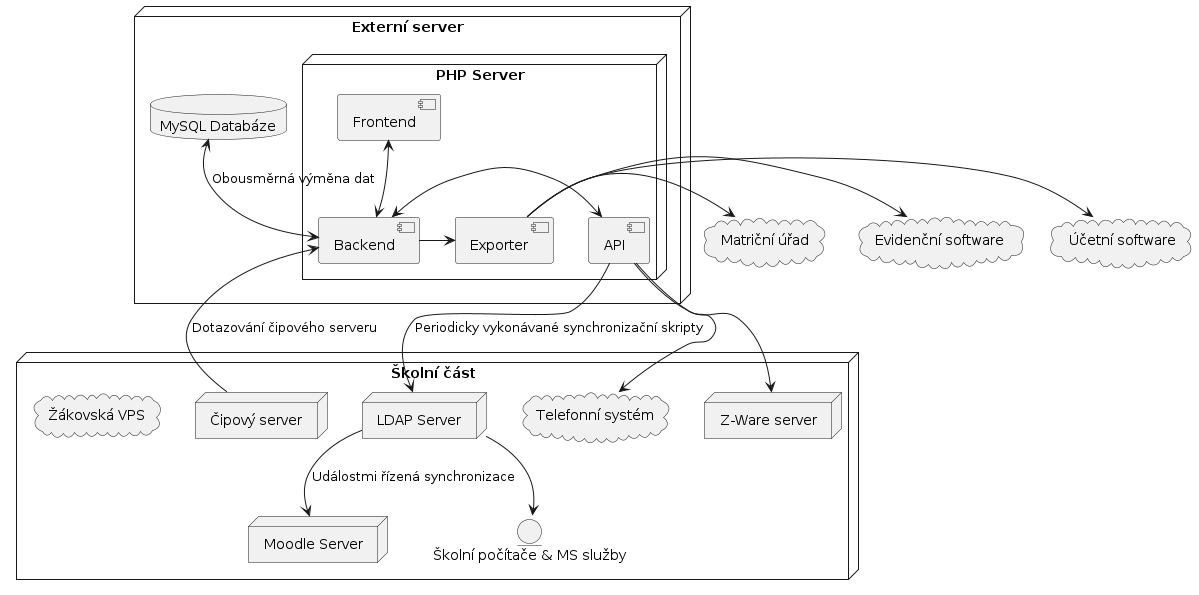
\includegraphics[width=\textwidth-28pt]{architektura-puvodni.png}
    \caption{Stávající architektura IS}
    \label{fig:architecture-old}
\end{figure}

% Miniobsah
% backend je množina skriptů napsaná v PHP, které se navzájem volají.

% Upravit co je co -> je všechno obláček
% Kdo za co odpovídá
% Barvy -> co patří škole, co patří jinam
% Zeleně -> ty, které mohu měnit
% Červeně -> nesáhnu

% Kde se software napojuje na software
% Jak vypadá struktura funkcí -> Kdo co určuje API? Ječná nebo Z-Ware?
% Kde se co realizuje, které inzeruji v výhodách IS
% Co musím mít a co by chceme mít
% Use case diagramy
% Sequence diag
% Jak se databáze plní ->
% KDe jsou formuláře? pouze ve frontendu?
% nejvyšší vrstva popisu databáze
% Kdo db dělá? jak by byl proces přidání nové komponenty?

Při pohledu na architekturu našeho ŠIS, vidím kombinaci vnějších a vnitřních služeb,
které spolu komunikují synchronizace dat mezi všemi službami, které IS poskytuje pro studenty,
rodiče, pedagogy i nepedagogické zaměstnance. Začněme tím, jak je konfigurován náš externí server.

Na externím serveru se nalézá relační databáze \textit{MySQL}, která slouží k uložení všech  
strukturovaných dat. Tato databáze je napojena na \textit{Backend} část, což je místo, kde probíhá
většina zpracování a řízení dat mezi databází a uživatelským rozhraním. Na tomto serveru je také
\textit{Frontend}, který je zodpovědný za vizuální prezentaci dat studentům, rodičům, pedagogickým i
nepegogickým zaměstnancům prostřednictvím webového prohlížeče. Na posledním bodu, máme zde \textit{API},
které slouží jako hlavní komunikační kanál mezi zmíněným backendem a dalšími službami,
jako je Moodle nebo LDAP.

Uvnitř školního areálu máme několik dalších klíčových služeb. \textit{LDAP Server}, který je
zodpovědný za centralizovanou autentizaci a autorizaci všech našich uživatelů v rámci školní
sítě a všech školních počítačů, na kterých běží operační systém Windows 10. Dále máme \textit{Moodle Server},
naši hlavní e-learningovou platformu, a \textit{Žákovská VPS}, 
virtuální privátní server pro studenty, na kterých se žáci učí operovat s Linuxovým prostředím,
jako jsou třeba webové aplikace (tj. konfigurace webových serverů), nebo další služby.
Linuxové VPS jsme zvolili na základě dat spolupráce s průmyslem. Naši školní partneři se vyjádřili,
že všichni, až na výjimky v počtu několika jedinců, využívají Linuxové servery pro svůj firemní záměr. 

Přehled o jednotlivých částí a jejich propojení jsem již zmínil. Nyní je třeba analýza jednitlivých rizik architektury.

\subsection*{Problematika Single Point of Failure}

Jedním z největších rizik v aktuální architektuře je \textit{Single Point of Failure (SPoF)} na straně PHP serveru. 
Pokud by tento server selhal, způsobilo by to výpadek většiny služeb, což by mělo vážné důsledky v celé škále případů. 

Dle architektury z diagramu \ref{fig:architecture-old} je viditelné, že v případě kdy by selhala celá externí část,
školní část může zcela bez problému fungovat s omezeními. LDAP server má vlastní databázový model pro ukládání dat, tedy
přihlášení na školních počítačích na síti nebude témeř vůbec ohroženo. Jediný případ, který mně napadá, je kdyby si uživatel
na externí části změnil heslo/některé údaje a LDAP se nestihl synchronizovat před selháním. To samé platí i pro Moodle
server, který si drží vlastní databázi uživatelů a dalších svých entit pro svou práci.
Třetí entitou ve školní části jsou \textit{Žákovská VPS}, avšak ty nejsou nijak propojena s IS.

Dalším dílem popisu jsou směry komunikace. Schéma znázorňuje, že mezi LDAP serverem a API je jednosměrné, tedy IS
LDAP může úpravy pouze přijímat. Důvod je jednoduchý: jakýkoliv zásah uživatele je zásahem do kritické části 
dat systému. K tomuto rozhodnutí - blokace obousměrné komunikace, vede bezpečnostní politika školy. Jakmile,
by si žák, nebo zaměstnanec mohl upravit například své jméno, upravil by tím citlivý záznam, který se následně
může propsat do matričních záznamů.

Z celého odstavce tedy vyplývá, že architekura kvůli své diverzifikaci je částečně ubráněna proti Single Point of Failure
a škola může i bez jedné či druhé části fungovat v omezeném režimu.

\section{Bezpečnost ŠIS}
Jak vyplývá z předchozí sekce, bezpečnost ŠIS a konzistence jeho je prioritou a tedy je
zaujat "default-deny" přístup, který má výchozí nastavení pro jakýkoliv přístup, operaci
nebo transakci zakázáno a povoluje explicitně ty operace nebo přístupy, které jsou
nezbytně nutné pro funkčnost systému nebo aplikace.

\subsection*{Jednosměrnost API \& matriční záznamy}  
Centrální jednotkou IS je Externí část schématu a její databázový model. Změny ze strany jiných služeb by mohl
být velice nebezpečný. IS 2x ročně (1x v říjnu a 1x v květnu) generuje svůj archivační model, který poskytuje
na žádost matričního úřadu.
Jakmile, by žák si například změnil své jméno v některém ze svých subsystémů, matriční úřad mohl přestat
párovat žáka v jeho občanské databázi a přestat evidovat jeho studium. V tomto případě by to mělo spoustu 
legislativních důsledků, jak lze vidět v schématu \ref{fig:dusledky-nestudia}

\begin{figure}[H]
    \centering
    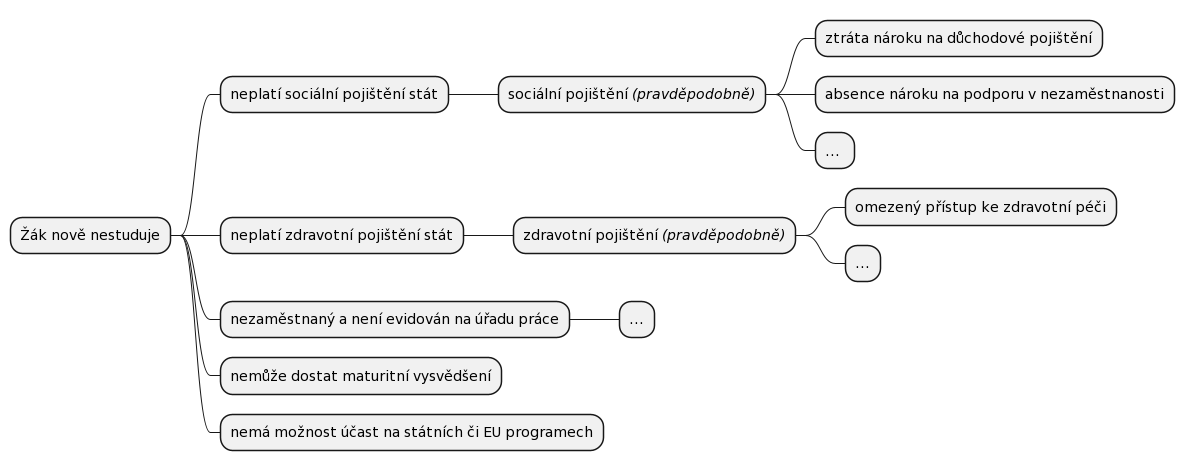
\includegraphics[width=\textheight-28pt, angle=90]{dusledky-nestudia.png}
    \caption{Následky zanechání studia v důsledku administrativní chyby}
    \label{fig:dusledky-nestudia}
\end{figure}

\section{Datové toky mezi komponentami}
\subsection*{Databáze a backend komponenty}
Mezi databázovým serverem a backendem webového serveru dochází k obousměrné výměně
dat. Backendová komponenta je jediná, která má přímý přístup do databázového serveru
a tedy kontroluje veškerá data, která IS shromažďuje, ukládá či poskytuje. Tato
vrstva na bezpečnostní funkci, zajišťuje konzistenci dat díky velkému množství
bezpečnostních procedur. Z backendové komponenty vystupují pouze další 3 komunikační
zdroje.

\subsection*{Backend a Frontend}
Uživatelské rozhraní (frontend) webové aplikace komunikuje s backendem přímo, aby získalo
potřebné informace nebo poslalo uživatelské vstupy přímo ke zpracování. Frontend je
tedy jediný způsob jediný způsob, jak přistoupit k datům uživatelsky přívětivou 
formou - formou webové stránky. Celá webová stránka je tedy generována metodou 
Server-Side-Rendering (SSR) - celý obsah stránky je seskládán
PHP skriptem do čisté HTML podoby a celý odeslán webovému clientu. Tento přístup zajišťuje
možnost manipulace s daty bez potřeby veřejného API. Pokud tedy pedagog, žák či 
rodič chce přistoupit například ke známkám žáka, musí jedině přes tento webový client.

Ředitel školy zastává názor, že veřejné API je velká bezpečnostní hrozba kvůli možném útokům
žáků. Většina žáků školy studuje obor Informační technologie a jsou tedy technologicky zdatní.
Žákovi tedy by stačilo znát veřejné API a příslušné dispozice výpočetního výkonu k DDoS útoku.
Školní systém se po dobu útoku stane nepoužitelným a zaměstnanci školy nemohou plnohodnotně
pracovat.

Zde se dají zúčastněným IS zobrazit informace:
\begin{itemize}
    \item novinky školy
    \item informace o osobě;
    \item seznam tříd, žáků, pedagogů, nepedagogických pracovníků, kontakty;
    \item známky;
    \item rozvrhy;
    \item detailní informace o SPU žáků;
    \item maturitní témata a okruhy;
    \item tématické plány předmětů;
    \item čipové záznamy příchodů a odchodů;
    \item a další...


\end{itemize}
Samozřejmostí je, že každá informace je řízena uživatelskými právy, tedy každý vidí pouze ty
informace, které ze zákona musí vědět.

\subsection*{Backend a Exporter}
Velkou částí IS je též Exporter. Je napsán jako PHP skript, který získává data z backendu a generuje
vyžadované datové sady. Nejdůležitější funkcionalitou je export dat pro Ministerstvo školství, mládeže 
a tělovýchovy (MŠMT), které spravuje matriční záznamy žáků ohledně jejich studia, jejich speciálních
potřeb a jejich následných vazeb. Jednou z takových vazeb může být platba statního zdravotního a 
sociálního pojištění.

MŠMT pořádá 2x ročně tzv. sběr\cite{skolni-matrika}, při kterých si vyžádá od školy,
(tedy ŠIS) snapshot ve formátu XML a se specifickým jménem a formátem o celé řadě 
dat o žácích školy. Každá úroveň státního školství má své specifické datum odevzdání.
Tyto informace poskytuje ministerstvo formou tabulky ve článku na svých stránkách
\cite{msmt-terminy-predavani-dat-2023}. Výjimkou je terciální vzdělávání, které probíhá
především na univerzitách. které se řídí dle SIMS - Sdružené informace matrik studentů.

Struktura souboru je dělena do položek, druhu kódování (tvaru zápisu),
druhu číselníku, typu dat, délce povoleného řetězce a povinnost záznamu.
 Uvedu výčet několika položek: % Vybírám tyto pro rozmatinost datové sady
\begin{itemize}
    \item datum sběru,
    \item IZO školy,
    \item rodné číslo žáka,
    \item pohlaví žáka,
    \item okres trvalého bydliště žáka,
    \item kvantifikátor státního občanství,
    \item nejvyšší stupeň vzdělání, kterého žák dosáhl před přijetím ke vzdělávání,
    \item ročník, ve kterém se žák vzděláván,
    \item obor vzdělání ve střední škole,
    \item způsob financování vzdělávání,
    \item kód 1. cizího studovaného jazyka
    \item ...
\end{itemize}
Tento výčet položek se avšak vztahuje pouze na žáky intaktní. Pro žáky se speciálními vzdělávacími
potřebami ministertvo vydává druhou sadu struktury datového rozhraní, která odpovídá specifickým
podmínkám těchto žáků. Tyto struktury dat jsou zvláště specifické pro každou úroveň vzdělávacího procesu,
od mateřských škol, po vyšší odborné.

Celý rejstřík položek, které vyžaduje MŠMT dále zpracovává a poskytuje pro Matriční úřad.

Problematikou implementace exporteru se zkomplikovává častou aktualizací datového rozhraní
pro předávání dat. Aktualizaci rozhraní vydává MŠMT přibližně jednou ročně, včetně aktualizace
číselníků\cite{msmt-rozhrani-predavani-dat-2023}. Možnost implementace se ještě zhoršuje kvůli formátu,
ve kterém ministerstvo poskytuje nové aktualizace. Formátem je PDF soubor ve článku na webu. Tento 
způsob tedy potřebuje vždy zásah do implementace člověkem a nelze nativně automatizovat.

Dalšími prvky, kam Exporter poskytuje data je evidenční software pro správu majetku školy a 
účetní software. Pro účetní software IS poskytuje data jako jsou například úvazky zaměstnanců,
pro kalkukaci výplat, příjmů a výdajů školy.

% Jak dobře je to napsaný? Lze nový export jednoduše dopsat?
% Konkrétnost -> 

\subsection*{Backend a Čipový server}
Backend je dále propojen s čipovým serverem, který eviduje příchody a odchody zaměstnanců a
žáků do a ze školy. Čipový server disponuje vlastní databází a poskytuje svá data pomocí API.
Čipový server má 2 zařízení pro evidenci příchodů a odchodů. Pro příchody je před dveřmi do školy
a pro odchody před dveřmi ze školy.  
Čipový server eviduje čísla karet, číslo záznamového zařízení a časy záznamů. 
Informační systém eviduje žáka a číslo jeho karty. 

% jak je to propojeno

\begin{figure}[H]
    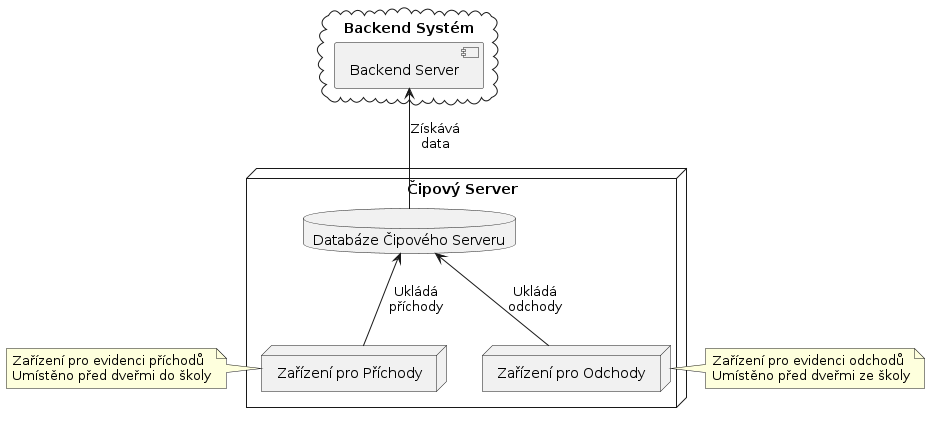
\includegraphics[width=\textwidth-28pt]{backend-cipovy-server.png}
    \caption{Schéma propojení záznamového systému čipových karet}
    \label{fig:backend-cipovy-server}
\end{figure}

\subsection*{Backend a API}
Backend systému je propojen pomocí neveřejného API s dalšími komponentami IS. Skryté API je 
uchováno pod speciální URL adresou se specifickým klíčem. Z tohoto API čerpají interní systémy,
především LDAP server, telefonní systém a Z-Ware.

Telefony (tj. systém telefonů) se dotazuje API pro přidělení linek ve škole a zajišťuje 
jejich konfiguraci. LDAP server se synchronizuje s API IS na základě periodicky vykonávaných
skriptů, obvykle 1x denně, případně lze i manuálně při údržbě.

Z-Ware je systém pro školní jídelnu. Ten si synchronizuje data sám, dle svého mechanismu
(garantuje externí firma). Data, která si synchronizuje jsou: čísla karet a čipů a žákovské 
účty, to jsou: username a heslo. Vše ostatní si řídí externí systém Z-Ware sám, včetně volby
obědů, záznamových zařízení, platby za obědy.

\begin{figure}[H]
    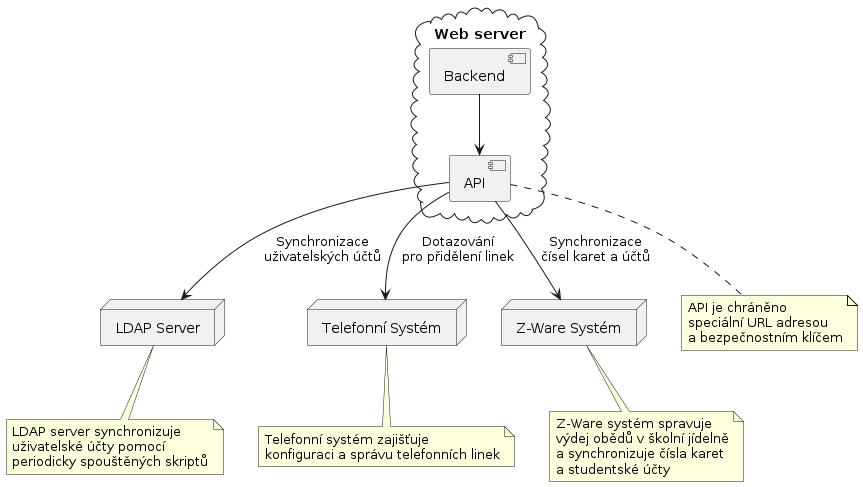
\includegraphics[width=\textwidth-28pt]{backend-api.png}
    \caption{Schéma připojení systémů na API}
    \label{fig:backend-api}
\end{figure}

\subsection*{LDAP server a Moodle}
Jednou z dalších částí je komunikace mezi LDAP serverem a Moodle serverem. Moodle je na škole
využíván jako hlavní nástroj pro celý e-learning a tedy je velmi důležitou součástí především
odborných předmětů, kam se umisťuje většina školních úloh nebo domáci úkolů.

Systém Moodle má modul, který umí synchronizovat uživatele a autentifikovat je u LDAP serveru.
To znamená, že pokud se uživatel (žák či zaměstnanec) chce přihlásit do Moodle, ten se 
autentifikuje uživatele LDAP protokolem u LDAP serveru a tím udržuje sychronizované účty právě
při události uživatele.
Vše lze řešit pomocí administrátora Moodle serveru, který může manuálně provést zavedení 
nových účtů a mazání starých či manuální synchronizaci.

Data, která se synchronizují jsou: jména, příjmení, email a třída. Pokud uživatel nemá třídu,
nepřiřazuje se a administrátor musí manuálně identifikovat uživatele. Vše ostatní, jako jsou 
zápisy do kurzů si řeší uživatelé sami. Moodle disponuje i vlastním ověřováním, avšak tento
mechanismus se používápouze  v ryze výjimečných případech, kdy chceme vytvořit účet i pro 
externí osobu.

\subsection*{LDAP server a školní počítače}
Veškeré počítače se autentifikují u LDAP serveru na domácí doméně SPSEJECNA.CZ. Jiné účty
na školních počítačích nejsou dovoleny z důvodu bezpečnosti.
Účet na školním Windows počítači se pouze u LDAP serveru autentifikuje. Žákovské, nebo
zaměstnanecké účty se ve škole nijak neliší. Jedinými synchronizovanými daty mezi školními
počítači a serverem jsou uživatelské disky na školních serverech.

\section{Databázový server a databázový model}
Současná databáze IS využívá MySQL verze 8.0.32 a její model \ref{fig:student-er-model}
disponuje 76 entitami, každá přidružená k některé z kategorií funcionalit, které IS disponuje.
Tabulka 

\begin{table}[H]
\begin{tabular}{lcl}
\hline
\multicolumn{1}{|l|}{\textbf{Druh}}                  & \multicolumn{1}{c|}{\textbf{Počet}} & \multicolumn{1}{l|}{\textbf{Užití}}                                                                                                                                       \\ \hline
\multicolumn{1}{|l|}{Žákovská správa}                & \multicolumn{1}{c|}{16}             & \multicolumn{1}{l|}{\begin{tabular}[c]{@{}l@{}}Identifikační údaje, rodiče, absence,\\ třídy, skupiny, certifikace, zdravotní\\ záznamy, specifické potřeby\end{tabular}} \\ \hline
\multicolumn{1}{|l|}{Zaměstnanecká správa}           & \multicolumn{1}{c|}{5}              & \multicolumn{1}{l|}{\begin{tabular}[c]{@{}l@{}}Identifikační údaje, typ úvazku,\\ třídnictví, kabinet\end{tabular}}                                                       \\ \hline
\multicolumn{1}{|l|}{Správa rozvrhů}                 & \multicolumn{1}{c|}{3}              & \multicolumn{1}{l|}{\begin{tabular}[c]{@{}l@{}}Úvazky zaměstnanců, rozvrhy \\ učeben, rozvrhy tříd\end{tabular}}                                                          \\ \hline
\multicolumn{1}{|l|}{Správa budovy}                  & \multicolumn{1}{c|}{2}              & \multicolumn{1}{l|}{\begin{tabular}[c]{@{}l@{}}Kabinety, učebny, technické místnosti,\\ kanceláře, správa kanceláří\end{tabular}}                                         \\ \hline
\multicolumn{1}{|l|}{Správa předmětů}                & \multicolumn{1}{c|}{5}              & \multicolumn{1}{l|}{Předměty, akreditace, tématické plány}                                                                                                                \\ \hline
\multicolumn{1}{|l|}{Správa souborového systému}     & \multicolumn{1}{c|}{3}              & \multicolumn{1}{l|}{\begin{tabular}[c]{@{}l@{}}Soubory k novinkám, certifikáty,\\ administrativní dokumenty\end{tabular}}                                                  \\ \hline
\multicolumn{1}{|l|}{Správa informací pro veřejnost} & \multicolumn{1}{c|}{3}              & \multicolumn{1}{l|}{\begin{tabular}[c]{@{}l@{}}Novinky, informace k přijímacímu \\ řízení, školní akce\end{tabular}}                                                      \\ \hline
\multicolumn{1}{|l|}{Správa školních akcí}           & \multicolumn{1}{c|}{4}              & \multicolumn{1}{l|}{\begin{tabular}[c]{@{}l@{}}Elektronické přihlašování na akce \\ pořádané školou\end{tabular}}                                                         \\ \hline
\multicolumn{1}{|l|}{Správa maturitních zkoušek}     & \multicolumn{1}{c|}{8}              & \multicolumn{1}{l|}{\begin{tabular}[c]{@{}l@{}}Data, účasti, místnosti, přepis \\ místností, maturitní projekty\end{tabular}}                                             \\ \hline
\multicolumn{1}{|l|}{Správa přijímacího řízení}      & \multicolumn{1}{c|}{2}              & \multicolumn{1}{l|}{\begin{tabular}[c]{@{}l@{}}Identifikační údaje, kola, ukončené\\ vzdělání, studijní výsledky\end{tabular}}                                            \\ \hline
\multicolumn{1}{|l|}{Spolupráce s průmyslem}       & \multicolumn{1}{c|}{2}              & \multicolumn{1}{l|}{\begin{tabular}[c]{@{}l@{}}Nabídky prací pro žáky, \\ spolupráce s průmyslem\end{tabular}}                                                            \\ \hline
\multicolumn{1}{|l|}{Číselníky MŠMT a NUTS}                 & \multicolumn{1}{c|}{15}             & \multicolumn{1}{l|}{\begin{tabular}[c]{@{}l@{}}Číselníky pro předávání \\ individuálních údajů ze školních\\ matrik státní správě, nomenklatura \\územních statistických jednotek\end{tabular}}                           \\ \hline
\multicolumn{1}{|l|}{Ostatní}                        & \multicolumn{1}{c|}{6}              & \multicolumn{1}{l|}{\begin{tabular}[c]{@{}l@{}}Číselné kódy zemí, anonymizační\\ číselníky, variabilní symboly bank \\bezpečnostní evidence\end{tabular}}                                         \\ \hline
\multicolumn{1}{r}{\textbf{SUMA}}                    & 74                                  &                                                                                                                                                                          
\end{tabular}
\caption{Evidence druhů entit v relačním modelu databáze}
\label{analysis:db-model}
\end{table}

\newpage

\subsection*{Žákovská správa}
Centrální součástí databázového modelu je modul Žákovské správy, který slouží
jako fundamentální základ pro shromažďování, zpracovávání a uchování
rozmanitých údajů o studentech. Ze schématu vyplývá, že

V jádru modulu stojí entita \textbf{Student}, která uchovává základní identifikační
a osobní údaje žáků, jako jsou jména, příjmení, data narození a další. Tato entita
je nepostradatelná pro jakékoli další operace a analýzy prováděné v rámci ŠIS. Její
důležitost vyplývá z její role, jako prinármího spojovacího bodu pro různé aspekty
školního života žáka.

Entita rodič, zahrnuje údaje o rodičích nebo zákonných zástupcích žáků. Umožňuje 
efektivní komunikaci mezi školou a rodinami a podporuje zapojení rodičů do školního
života jejich dětí kvůli přihlašování do systému. Záznamy o rodičích jsou zásadní pro
posílení rodinného zapojení ve školním vzdělávacím procesu a poskytují oporu při
kázeňských problémech.

Entita třída reprezentuje uspořádání a přiřadení studentů do konkrétních tříd a 
studijních skupin. Tato etntita je základem pro organizaci předmětů, učitelů,
učeben, nebo třeba zápisu známek. Propojení studentů s konkrétními třídami je 
klíčové pro správu a plánování školních aktivit.

Entity Známky a Certifikace se zaměřují na sledování a hodnocení 
výsledků žáků. Tyto entity zahrnují informace o studijních výsledcích v
jednotlivých předmětech. Dále entity spravují odborné či jazykové certifikace,
které žáci mohou získat během studia a tím nechat uznat například praktickou
maturitní zkoušku.

Absence žáků je klíčovou rolí v monitorování a správě školní docházky. 
Zaznamenává dobu neúčasti žáků na vyučování v jednotlivých dnech a na 
předmětech, což je zásadní pro identifikaci a řešení problémů s docházkou.
Systém absence přímo odkazuje na entitu Student prostřednictvím cizího klíče,
což umožňuje přesné sledování a analýzu absencí každého jednotlivého žáka.

Zdravotní pojištění je další z entit a obsahuje důležité informace o zdravotní
péči a pojištění žáků. Tato entita umožňuje škole sledovat zdravotní pojištění
žáků, což se hodí pro zajištění dalších procesů v případě zdravotních
problémů.

Diagram databázového modelu je zjednodušený snížení komplexity diagramů.
\begin{figure}[H]
    \includegraphics[height=\textheight-28pt]{student-er-model1.png}
    \caption{Zjednodušený diagram databázového modelu modulu Žákovské správy}
    \label{fig:student-er-model}
\end{figure}

% Napsat do firem kolik škol to využívá

\subsection*{Server-side-rendering a Client-side-rendering}

Z analýzy našeho informačního systému vyplývá, že vhodná kombinace obou přístupů může 
přinést optimalizovaný a bezpečný uživatelský zážitek. V kontextu akademických aplikací
je klíčové zajistit bezpečnost a integritu dat, zatímco je stále třeba poskytovat 
rychlý a plynulý uživatelský zážitek.

V závěru, rozhodnutí o výběru mezi client-side a server-side scripting,
stejně jako mezi SSR a CSR, by mělo být učiněno s ohledem na specifické potřeby a omezení 
daného projektu. V kontextu našeho informačního systému je klíčové nalézt správnou 
rovnováhu mezi výkonem, bezpečností a uživatelským zážitkem.

Ječná IS, disponuje plně Server-Side-Renderingem, kde se všechna data sestavují na straně
PHP serveru - Externí část architektury. Dle iniciálního benchmarkingu se zjistilo, že
některé operace umí databázový systém MySQL renderovat rychleji, než samotné PHP s rozdílem
desítek procent. Tedy Ječná IS některé informace renderuje na již na straně databáze. 
Konkrétním příkladem jména žáků spojená s jejich třídami.

\subsection*{Konkrétní příklad}
...


\section{Funkce API a uživatelské rozhraní}
\section{Identifikace a analýza potřeb koncových uživatelů}
\section{Hodnocení výhod a nevýhod in-house vývoje informačního systému}

\chapter{Návrh nového systému}
\section{Detaily nově navrženého systému}
\section{Zapojení potřeb uživatelů a moderních trendů v IT}
\section{Proces modernizace}

\chapter{Diskuse}
\section{Porovnání výsledků s původními hypotézami a otázkami výzkumu}
\section{Interpretace výsledků}
\section{Diskuze omezení výzkumu a možností dalšího vývoje}

\chapter{Závěr}
\section{Shrnutí klíčových zjištění}
\section{Závěrečné úvahy a doporučení pro budoucí praxi a práce}

\chapter{Reference}
\printbibliography[heading=none]

\chapter{Přílohy}


\end{document}
